\documentclass[tikz]{standalone}
\usepackage{pgfplots}
\pgfplotsset{compat=1.15}
\usepackage{mathrsfs}
\usetikzlibrary{arrows,calc}
\usepackage{tkz-euclide}
\pagestyle{empty}

\definecolor{AngleClr}{rgb}{0,0.39215686274509803,0}
\definecolor{ShapeClr}{rgb}{0.6,0.2,0}

\begin{document}

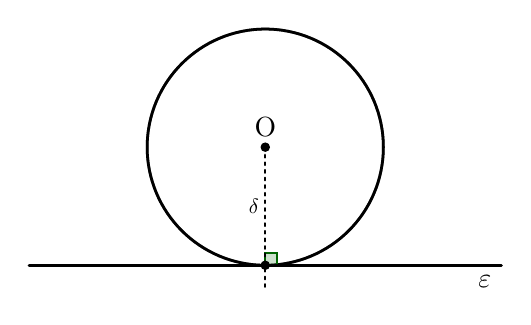
\begin{tikzpicture}[scale=.75]
\tkzSetUpLine[line width=1pt,color=black]
\tkzSetUpPoint[fill=black]

\tkzDefPoints{0/0/O,2/0/A,-4/-2/B,4/-2/C,0/-2/D}


\tkzDrawCircle[line width=1.0pt,fill=white](O,A)
\tkzDrawCircle[line width=1.0pt,draw=black](O,A)
\tkzMarkRightAngles[line width=0.75pt, size=.2,color=AngleClr,fill=AngleClr,fill opacity=0.2](O,D,C)
\tkzDrawSegments[line width=1pt,color=black](B,C)
\tkzDrawSegments[line width=0.75pt,color=black,dashed,dash pattern=on 1pt off 1.75pt, add=0 and 0.2](O,D)


\tkzDrawPoints[size=3](O,D)
\tkzLabelPoint[above](O){$\rm O$}
\tkzLabelPoint[below left](C){$\varepsilon$}

\tkzLabelSegment[left=-0.05](O,D){\scalebox{0.75}{$\delta$}}

\end{tikzpicture}
\end{document}
